\section{AWS cost}
\label{sec:AWS cost}

Nei capitoli successivi vedremo quali servizi AWS sono stati adottati e soprattuto in che modo sono stati sfruttati nella creazione della piattaforma, come accennato in questa parte ci concentreremo invece solo sull’analisi dei costi.
Le tabelle seguenti conterranno i dati raccolti dai listini prezzi di AWS, questi successivamente saranno elaborati per stimare il costo mensile e annuale necessario per la realizzazione dell’intera piattaforma.
I dati seguenti si basano su alcune assunzioni derivanti dal caso d’uso d’interesse e permettono una interpretazione più rapida e comprensibile:
\begin{itemize}
\item I video durano in media 5 minuti
\item Le dimensioni dei video cambiano a seconda della qualità :

\begin{table}[h!]
\centering
\begin{tabular}{ |p{3cm}|p{3cm}|p{3cm}|  }
  \hline
  \multicolumn{3}{|c|}{Cost for minute} \\
  \hline
  Minute & Quality & Cost \\
  \hline
  1 & SD & 0.01185185185 \\
  1 & SD & 0.08 \\
  \hline
\end{tabular}
\caption{Table of cost for minute}
\label{table:1}
\end{table}

\begin{table}[h!]
\centering
\begin{tabular}{ |p{3cm}|p{3cm}|p{3cm}|  }
  \hline
  \multicolumn{3}{|c|}{Gb for a video} \\
  \hline
  Video & Quality & Gb \\
  \hline
  1 & SD & 0.05925925926 \\
  1 & HD & 0.4 \\
  \hline
\end{tabular}
\caption{Table of Gb for a video}
\label{table:1}
\end{table}


\item Il costo della transcodifica e quindi del servizio dell’Elastic Transcoder è di:

\begin{table}[h!]
\centering
\begin{tabular}{ |p{3cm}|p{3cm}|p{3cm}|  }
  \hline
  \multicolumn{3}{|c|}{Elastic Transcoder cost for minute} \\
  \hline
  Minute & Quality & Cost \\
  \hline
  1 & SD & 0.0185 \\
  1 & SD & 0.037 \\
  \hline
\end{tabular}
\caption{Table of cost for minute}
\label{table:1}
\end{table}

\begin{table}[h!]
\centering
\begin{tabular}{ |p{3cm}|p{3cm}|p{3cm}|  }
  \hline
  \multicolumn{3}{|c|}{Elastic Transcoder cost for a video} \\
  \hline
  Video & Quality & Cost \\
  \hline
  1 & SD & 0.0925 \\
  1 & HD & 0.185 \\
  \hline
\end{tabular}
\caption{Table of cost for a video}
\label{table:1}
\end{table}


\item Il costo dello storage dei video su S3 è di 0.03\$/GB
\item Il costo per il trasferimento è di :


\begin{table}[h!]
\centering
\begin{tabular}{ |p{3cm}|p{3cm}|p{3cm}|  }
  \hline
  \multicolumn{2}{|c|}{Network traffic} \\
  \hline
  TB & Cost per GB \\
  \hline
  10 & 0.09 \\
  40 & 0.08 \\
  100 & 0.06 \\
  350 & 0.04 \\
  524 & 0.03 \\
  4000 & 0.03 \\
  5000 & 0.02 \\
  \hline
\end{tabular}
\caption{Table of network traffic cost}
\label{table:1}
\end{table}


\end{itemize}

Raccolti i costi dei vari servizi utilizzati in X-Learning, come accennato precedentemente ora ci focalizziamo nel calcolo di alcune stime sulla base dei numero dei video e del numero di visualizzazioni:
Costo per lo storage su S3 e la transcodifica è di:


\begin{table}[h!]
\begin{tabular}{ |p{2cm}|p{2cm}|p{2cm}|p{2cm}|p{2cm}| }
  \hline
  \multicolumn{5}{|c|}{S3 and Elastic Transcoder} \\
  \hline
  video & S3 month & S3 year & Elastic Transcoder & Total \\
  \hline
  100 & 1.2 & 14.4 & 18.5 & 32.9\\
  1000 & 12 & 144 & 185 & 329\\
  10000 & 120 & 1440 & 1850 & 3290\\
  50000 & 600 & 7200 & 9250 & 16450\\
  100000 & 1200 & 14400 & 18500 & 32900\\
  500000 & 6000 & 72000 & 92500 & 164500\\
  1000000 & 12000 & 144000 & 185000 & 329000\\
  \hline
\end{tabular}
\caption{Table of total cost per storage and transcoder}
\label{table:1}
\end{table}

Costo dello Streaming di qualità SD è di:

\begin{table}[h!]
\begin{tabular}{ |p{2cm}|p{2cm}|p{2cm}|p{2cm}|p{2cm}| }
  \hline
  \multicolumn{5}{|c|}{SD Streaming cost} \\
  \hline
  views & minute & gb & cost/month & single video cost\\
  \hline
1,000 & 5,000 & 59.26 & 5.04 & 0.00504\\
10,000 & 50,000 & 592.59 & 50.37 & 0.00504\\
50,000 & 250,000 & 2,962.96 & 251.85 & 0.00504\\
100,000 & 500,000 & 5,925.93 & 503.70 & 0.00504\\
500,000 & 2,500,000 & 29,629.63 & 2,420.37 & 0.00484\\
1,000,000 & 5,000,000 & 59,259.26 & 4,605.56 & 0.00461\\
5,000,000 & 25,000,000 & 296,296.30 & 15,901.85 & 0.00318\\
10,000,000 & 50,000,000 & 592,592.59 & 26,827.78 & 0.00268\\
  \hline
\end{tabular}
\caption{Table of SD Streaming cost}
\label{table:1}
\end{table}


Costo dello streaming di qualità HD è di:

\begin{table}
\centering 
\begin{tabular}{ |p{2cm}|p{2cm}|p{2cm}|p{2cm}|p{2cm}| }
  \hline
  \multicolumn{5}{|c|}{HD Streaming cost} \\
  \hline
  views & minute & gb & cost/month & single video cost\\
  \hline
1,000 & 5,000 & 400 & 34 & 0.034 \\
10,000 & 50,000 & 4,000 & 340 & 0.034\\
50,000 & 250,000 & 20,000 & 1650 & 0.033\\
100,000 & 500,000 & 40,000 & 3250 & 0.0325\\
500,000 & 2,500,000 & 200,000 & 12050 & 0.0241\\
1,000,000 & 5,000,000 & 400,000 & 20050 & 0.02005\\
5,000,000 & 25,000,000 & 2,000,000 & 64170 & 0.012834\\
10,000,000 & 50,000,000 & 4,000,000 & 114170 & 0.011417\\
  \hline
\end{tabular}
\caption{Table of HD Streaming cost}
\label{table:1}
\end{table}

I dati appena illustrati possono essere sintetizzati attraverso l’ausilio di alcuni grafici:


\begin{figure}[htb]
 \centering
 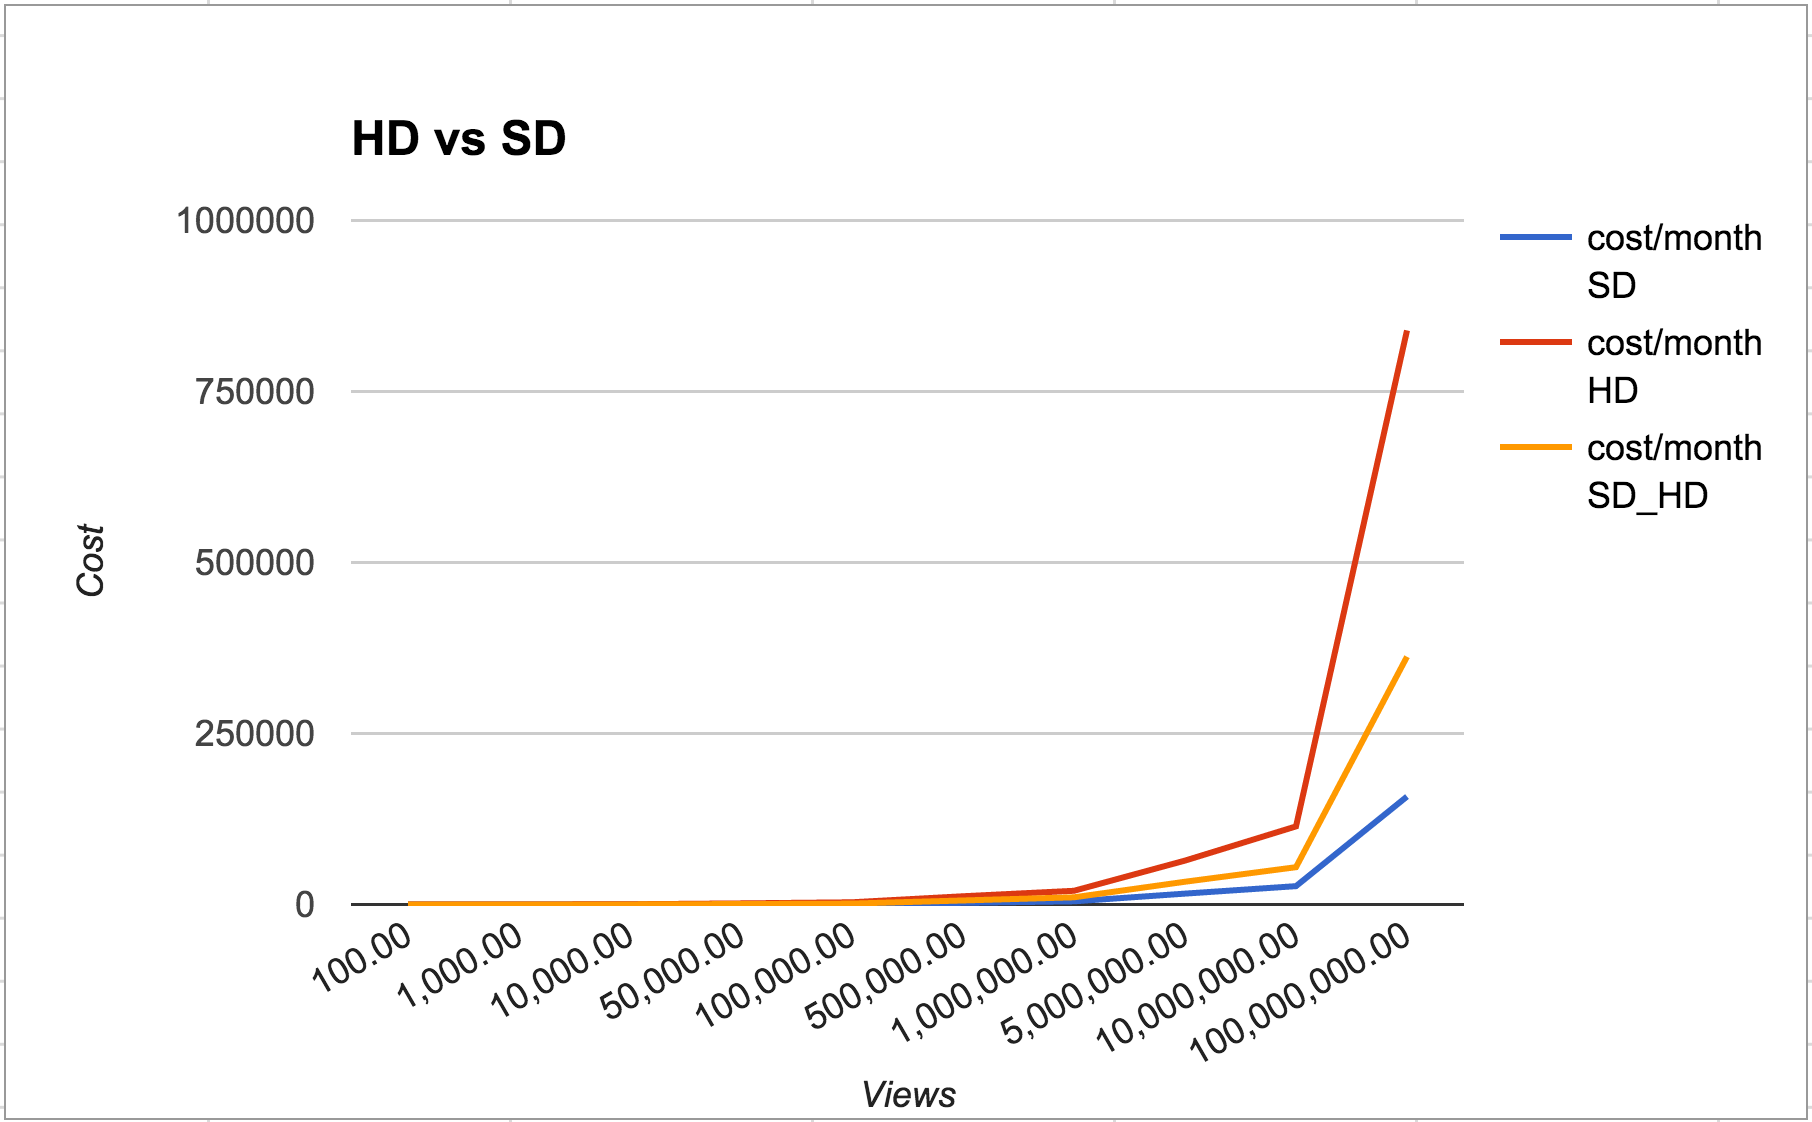
\includegraphics[width=1.0\linewidth]{images/chapter3/grafico.png}\hfill
 \caption[xxxxxxx]{xxxxxxx}
 \label{fig:fourV}
\end{figure}
